\documentclass[10pt,t,english,aspectratio=1610]{beamer}
\usepackage{fontawesome}
\usepackage{graphicx}
\usepackage{array}
\usepackage[normalem]{ulem}
\usepackage{amsfonts,amsmath,amssymb,bm,bbm}
\usepackage{mathrsfs}
% NOTE: sgame is intentionally NOT used -- its `game` environment is
% incompatible with the `array` package (required by colortbl/makecell/multirow)
% and errors with "Missing # inserted in alignment preamble". We use the modern
% TikZ-based `xgames` package instead (loaded after TikZ below).
\usepackage{graphicx,pstricks}
\usepackage{xcolor}
\usepackage{colortbl}
\usepackage{makecell}
\usepackage{tikz,tikzsymbols,gnuplottex}
\usetikzlibrary{decorations.pathreplacing,shapes,positioning,arrows.meta,fit,backgrounds,calc}

% --- xgames: TikZ-based game-theory typesetting (matrixgame, gametree,
% beliefspace, automaton). Not on CTAN; xgames.sty + fikz.sty are vendored at
% the repo root. CC BY-SA 4.0 (xgames) / GPL-3.0 (fikz), (c) Benjamin Bernard.
\usepackage{xgames}

% Custom command for shading rows in a matrixgame
% ---------------------------------------------------------------------------
% \shaderow[<fill options>]{<row>}{<first column>}{<last column>}
% Call this inside the matrixgame, after \payoffmatrix
% Can wrap in a \foreach to shade multiple regions
% Example: \foreach \i in {1,...,5}{ \shaderow[green!50!black]{\i}{\i}{5} }
\newcommand{\shaderow}[4][red!60]{%
  \ifnum#3=1\relax\def\xl{0}\else\pgfmathsetmacro{\xl}{\pmtwi[#3-1]}\fi
  \ifnum#2=1\relax\def\yt{0}\else\pgfmathsetmacro{\yt}{\pmthi[#2-1]}\fi
  \pgfmathsetmacro{\xr}{\pmtwi[#4]}%
  \pgfmathsetmacro{\yb}{\pmthi[#2]}%
  \fill[opacity=0.18, #1] ($(pmt1-tl)+(\xl,-\yt)$) rectangle ($(pmt1-tl)+(\xr,-\yb)$);%
}

\usepackage[english]{babel}
\usepackage[utf8]{inputenc}
\usepackage{appendixnumberbeamer}
\usepackage{datetime2}
\usepackage{booktabs}
\usepackage{setspace}
\usepackage{rotating}
\usepackage{multirow}
\usepackage{listings}

\usepackage{natbib}
\bibliographystyle{unsrtnat}
\renewcommand{\bibfont}{\footnotesize}
\renewcommand{\bibsection}{\vspace{-1em}}

%\usepackage{matlab-prettifier} % For enhanced MATLAB highlighting
\lstset{
    language=matlab,
    % Other options for styling (optional)
    basicstyle=\ttfamily\footnotesize, % Font style
    keywordstyle=\color{blue}, % Keyword color
    commentstyle=\color{green!50!black}, % Comment color
    stringstyle=\color{red!70!black}, % String color
    numbers=left, % Line numbers on the left
    numberstyle=\tiny\color{gray}, % Style for line numbers
    frame=single, % Frame around the listing
    breaklines=true, % Allow line breaking
    captionpos=b, % Caption at the bottom
    tabsize=4 % Tab size
}

% ------------------------------------------------------------------------------
% Use the beautiful metropolis beamer template
% ------------------------------------------------------------------------------
\usepackage[T1]{fontenc}
\usepackage[utf8]{inputenc}
\usepackage{fontawesome}
\usepackage{FiraSans} 
\mode<presentation>
{
  \usetheme[progressbar=foot,background=light]{metropolis} 
  \usecolortheme{default} % or try albatross, beaver, crane, ...
  \usefonttheme{default}  % or try default, serif, structurebold, ...
  \setbeamertemplate{navigation symbols}{}
  \setbeamertemplate{caption}[numbered]
  %\setbeamertemplate{frame footer}{My custom footer}
  \makeatletter
    \setbeamertemplate{frametitle continuation}{}
  \makeatother
} 
\addtobeamertemplate{frametitle continuation}{}{%
  \setbeamertemplate{frametitle continuation}{}%
}
\setbeamertemplate{frametitle continuation}{}

\newenvironment{stepenumerate}{\begin{enumerate}[<+->]}{\end{enumerate}}
\newenvironment{stepitemize}{\begin{itemize}[<+->]}{\end{itemize} }
\newenvironment{stepenumeratewithalert}{\begin{enumerate}[<+-| alert@+>]}{\end{enumerate}}
\newenvironment{stepitemizewithalert}{\begin{itemize}[<+-| alert@+>]}{\end{itemize} }

\newtheorem{question}{Question}
\newtheorem{claim}{Claim}
\newtheorem{proposition}{Proposition}
\newtheorem{remark}{Remark}
\newtheorem{conjecture}{Conjecture}

\definecolor{metrop}{RGB}{29, 44, 44}
\colorlet{GrayLight}{black!15}
\colorlet{GrayMedium}{black!30}
\colorlet{ForestGreen}{green!60!black}

\newenvironment{transitionframe}{
  \setbeamercolor{background canvas}{bg=black!80}
  \begin{frame}}{
    \end{frame}
}

\newcommand{\bsk}{

\bigskip

}

\newcommand{\pd}{\partial}
\newcommand{\RR}{\mathbb{R}}

\newcommand*\hugme[1]{\tikz[baseline=(char.base)]{\node[shape=ellipse,draw,inner sep=0pt] (char) {#1};}}

\newcounter{saveenumi}
\newcommand{\seti}{\setcounter{saveenumi}{\value{enumi}}}
\newcommand{\conti}{\setcounter{enumi}{\value{saveenumi}}}
\resetcounteronoverlays{saveenumi}



\newcommand\dotprod[2]{\langle #1 , #2 \rangle}
\newcommand{\ft}[1]{\widehat #1}
\newcommand{\qabove}[1]{\overset{\text{\large \textbf ?}}{#1}}
\newcommand{\eqae}{\overset{\text{a.e.}}{=}}
\newcommand{\calp}{\mathcal{P}}
\newcommand{\calg}{\mathcal{G}}
\newcommand{\calb}{\mathcal{B}}
\newcommand{\textd}{\text{d}}
\newcommand{\bbr}{\mathbb{R}}
\newcommand{\binm}{\mathbin{M}}
\newcommand{\binc}{\mathbin{C}}
\newcommand{\binb}{\mathbin{B}}
\newcommand{\calc}{\mathcal{C}}
\newcommand{\calh}{\mathcal{H}}
\newcommand{\bfone}{\mathbf{1}}
\newcommand{\bbe}{\mathbb{E}}
\newcommand{\bfle}{\mathbf{e}}
\newcommand{\calf}{\mathcal{F}}
\newcommand{\cala}{\mathcal{A}}
\newcommand{\cale}{\mathcal{E}}
\newcommand{\bbn}{\mathbb{N}}
\newcommand{\cantor}{\calc}
\newcommand{\calY}{\mathcal{Y}}
\newcommand{\textb}{\text{B}}
\newcommand{\calm}{\mathcal{M}}
\newcommand{\bint}{\mathbin{T}}
\newcommand{\ep}{\epsilon}
\newcommand{\bbq}{\mathbb{Q}}
\newcommand{\bbp}{\mathbb{P}}
\newcommand{\cals}{\mathcal{S}}
\newcommand{\emptysequence}{e}
\newcommand{\bbz}{\mathbb{Z}}
\newcommand{\fraka}{\frak{A}}
\newcommand{\frakb}{\frak{B}}
\newcommand{\length}{\text{length}}
\newcommand{\bfn}{\mathbf{N}}
\newcommand{\support}{\text{support}}
\DeclareMathOperator*{\argmax}{arg\,max}
\newcommand{\dom}{\mbox{dom}}
\def\ut{\underline t}
\def\um{\underline m}
\def\PP{\mathbb{P}}
\def\EE{\mathbb{E}}
\def\RR{\mathbb{R}}

% Title page info
\title[Weak Sequential Equilibrium]{Chapter 11: Weak Sequential Equilibrium}
\author[ECON 5001]{ECON 5001\\Prof. Paul J. Healy\\Based on: \textit{Game Theory} by Giacomo Bonanno} \color{metrop}
\institute[OSU]{}
\date[]{\vfill {\tiny Updated \today\ at\ \DTMcurrenttime}}

% ---------------------------------------------------------------------
% SCOPE AND NOTATION
%   Lite Chapter 11: assessment (sigma, mu), sequential rationality,
%   Bayesian updating at reachable info sets, WSE, WSE => NE, existence,
%   WSE is not always SPNE (Venn diagram). Sequential equilibrium
%   (Ch 12) is only previewed, never defined.
%   Bonanno's formal pi_i(H | sigma, mu) notation is skipped.
%   Bayesian updating uses Bayes' rule from deck 11.
%
% ANSWERS (all checked numerically)
%   Donut Truck. Truck (entrant): Out, Cart, Premium. Buckeye Donuts
%   (incumbent) sees entry, not the plan: Fight or Accommodate.
%   Payoffs (Truck, Buckeye):
%     Out (0,4). Cart: F (-1,3), A (1,2). Premium: F (-2,0), A (3,1).
%   No proper subgames, so SPNE = NE = {(Out, Fight), (Premium, Acc)}.
%   mu = Pr(Cart | entry). Fight: 3 mu. Acc: 2 mu + 1(1-mu) = 1 + mu.
%     Fight best iff mu >= 1/2.
%   Mix Out 1/2, Cart 1/10, Premium 2/5: mu = (1/10)/(1/2) = 1/5.
%   WSE: (Premium, Acc) with mu = 0. (Out, Fight) with any mu >= 1/2.
%   Selten's horse WSE: (a,e,c) and (b,e,c). Not (a,f,c): f gives P2
%     1 < 2 from e. Not (b,f,d): d strictly dominated at P3's info set.
%   Herding (60% majority, equal priors, players follow own signal):
%     P2 after Blue guess + own blue: .36/(.36+.16) = 9/13 = .69.
%     P3 after Blue, Blue + own red: .6 -> guess Blue anyway (cascade).
%   Worked example (Dead Phones). Alex: Cancel (2,2), or go to
%   Cazuela's / Yoshi. Blair can't tell which: C, M (Massey's), Y, H.
%     At Cazuela's: C (4,3)  M (1,2)  Y (0,0)  H (0,1)
%     At Yoshi:     C (0,0)  M (1,2)  Y (3,3)  H (0,1)
%     Pure NE: (Cancel, M), (Cancel, H), (Caz, C), (Yoshi, Y).
%     mu = Pr(Caz). Blair: C 3mu, M 2, Y 3(1-mu), H 1.
%     WSE: (Caz, C) mu=1; (Yoshi, Y) mu=0; (Cancel, M) mu in [1/3,2/3].
%     (Cancel, H) is never part of a WSE (H < M always).
%     Alex mixes Cancel 1/2, Caz 1/3, Yoshi 1/6: mu = 2/3.
%       Blair: C 2, M 2, Y 1, H 1 -> C or M (tie).
% ---------------------------------------------------------------------

% Selten's horse (Bonanno Figure 7.12 / 11.9), copied from deck 09
\newcommand{\horse}[1][]{%
\begin{tikzpicture}[>=Stealth, scale=0.95,
    dot/.style={circle, fill, inner sep=1.7pt},
    pay/.style={align=center, font=\small, inner sep=1pt}]
  \node[dot] (n1) at (0,0) {};
  \node[dot] (n2) at (3.2,0) {};
  \node[dot] (t)  at (5.8,0) {};
  \node[dot] (x)  at (0,-1.9) {};
  \node[dot] (y)  at (3.2,-1.9) {};
  \node[font=\large, text=player1, above=3pt] at (n1) {1};
  \node[font=\large, text=player2, above=3pt] at (n2) {2};
  \draw[->, thick] (n1) -- node[above] {$b$} (n2);
  \draw[->, thick] (n2) -- node[above] {$f$} (t);
  \draw[->, thick] (n1) -- node[left] {$a$} (x);
  \draw[->, thick] (n2) -- node[left] {$e$} (y);
  \node[pay, right=3pt] at (t.east) {\textcolor{player1}{1}\\\textcolor{player2}{1}\\\textcolor{player3}{0}};
  \draw[thick, rounded corners=7pt, player3] ($(x)+(-0.4,0.3)$) rectangle ($(y)+(0.4,-0.3)$);
  \node[font=\large, text=player3] at ($(x)!0.5!(y)$) {3};
  \foreach \n/\s in {x/0, y/3.2}{
    \node[dot] (\n c) at (\s-0.7,-3.5) {};
    \node[dot] (\n d) at (\s+0.7,-3.5) {};
    \draw[->, thick] (\n) -- node[left] {$c$} (\n c);
    \draw[->, thick] (\n) -- node[right] {$d$} (\n d);
    \node[pay, below=2pt] at (\n c.south) {\textcolor{player1}{2}\\\textcolor{player2}{2}\\\textcolor{player3}{2}};
    \node[pay, below=2pt] at (\n d.south) {\textcolor{player1}{0}\\\textcolor{player2}{0}\\\textcolor{player3}{0}};
  }
  #1
\end{tikzpicture}}

% The Donut Truck. #1 = scale, #2 = extra options/overlays on the tree
\newcommand{\donuttree}[2][0.85]{%
\begin{gametree}[player names={Truck, Buckeye Donuts}, scale=#1]
  \branch[player=1, root=w, label=90] from (0,0) to[v=1.4, h=3.6] {Out(0,4); Cart; Premium};
  \branch[player=2, label=none] from (w2) to[v=1.6, h=1.7] {Fight(-1,3); Acc(1,2)};
  \branch[label=none] from (w3) to {Fight(-2,0); Acc(3,1)};
  \informset (w2) -- (w3);
  #2
\end{gametree}}

% Dead Phones (worked example)
\newcommand{\phonetree}[1][0.7]{%
\begin{gametree}[player names={Alex, Blair}, scale=#1]
  \branch[player=1, root=w, label=90] from (0,0) to[v=1.3, h=5.4] {Cancel(2,2); Caz; Yoshi};
  \branch[player=2, label=none] from (w2) to[v=2.2, h=1.5] {C(4,3); M(1,2); Y(0,0); H(0,1)};
  \branch[label=none] from (w3) to {C(0,0); M(1,2); Y(3,3); H(0,1)};
  \informset (w2) -- (w3);
\end{gametree}}

\begin{document}

\frame{\maketitle}

\begin{frame}{Where We Left Off: Selten's Horse}
\begin{columns}[c]
\begin{column}{0.5\textwidth}
\centering
\horse
\end{column}
\begin{column}{0.48\textwidth}
Four pure NE. All are SPNE:\\[4pt]
$(a,e,c)$ \quad $(a,f,c)$\\[2pt]
$(b,e,c)$ \quad $(b,f,d)$
\bsk
SPNE only checks \textbf{subgames}
\begin{itemize}
    \item P3's info set isn't a subgame
    \item So bad choices there go unchecked
\end{itemize}
\bsk
\onslide<2->{\textbf{Fix:} give P3 a \textbf{belief} about where she is. Check every choice against it}
\end{column}
\end{columns}
\vspace{-0.3in}
\end{frame}

% ---- MobLab run: Herding (Information Cascade) ------------------------
% Macro and Finance topic. Default majority 60%. Groups of 5-6, random
% order. A few periods. Play BEFORE beliefs are defined. Results come
% back in "Back to Herding".
% ---------------------------------------------------------------------
\begin{frame}{MobLab: ``Herding (Information Cascade)''}
\begin{itemize}
    \item MobLab time!
    \item A jar is either mostly \textbf{Blue} or mostly \textbf{Red} (equally likely)
    \begin{itemize}
        \item Mostly $=$ 60\% of the balls
    \end{itemize}
    \item You privately draw one ball (it goes back in)
    \item One at a time, in random order, guess: Blue jar or Red jar?
    \begin{itemize}
        \item You see everyone's \textbf{guesses} before you. Not their balls
    \end{itemize}
    \item Paid for a correct guess
\end{itemize}
\vfill
\centering
Feel free to talk! And play it the way you'd actually play it.
\vspace{-0.2in}
\end{frame}

% ==============================================================
% 11.1 ASSESSMENTS AND SEQUENTIAL RATIONALITY
% ==============================================================

\begin{frame}[standout]
Beliefs at Information Sets
\end{frame}

\begin{frame}{Example: The Donut Truck}
A new donut truck thinks about parking near Buckeye Donuts on High St
\begin{itemize}
    \item \textbf{Out}: stay away
    \item \textbf{Cart}: a cheap little cart (weak)
    \item \textbf{Premium}: a full truck with a big menu (strong)
\end{itemize}
\bsk
Buckeye Donuts sees \textbf{that} the truck showed up, not \textbf{which} plan
\begin{itemize}
    \item \textbf{Fight}: price war. \ \textbf{Acc}: accommodate
    \item Fighting a weak cart pays. Fighting a strong truck doesn't
\end{itemize}
\vspace{-0.3in}
\end{frame}

\begin{frame}{The Donut Truck}
\begin{columns}[c]
\begin{column}{0.5\textwidth}
\centering
\donuttree{}
\end{column}
\begin{column}{0.48\textwidth}
\centering
\begin{matrixgame}[top={Fight, Acc}, left={Out, Cart, Premium}, player names={Truck, Buckeye}, br=<2->]
  \payoffmatrix{0,4 & 0,4 \\ -1,3 & 1,2 \\ -2,0 & 3,1}
\end{matrixgame}
\end{column}
\end{columns}
\bsk
Proper subgames? \underline{\hspace{0.5in}} \ So $SPNE=NE$
\bsk
\onslide<2->{NE: \underline{\hspace{1in}} \quad \underline{\hspace{1in}}}
\bsk
\onslide<3->{Is (Out, Fight) reasonable? \ \textbf{It depends on what Buckeye believes}}
\vspace{-0.3in}
\end{frame}

\begin{frame}{What Should Buckeye Believe?}
\begin{columns}[c]
\begin{column}{0.48\textwidth}
\centering
\donuttree[0.78]{\node[font=\small] at ($(w2)+(-0.15,0.35)$) {$\mu$}; \node[font=\small] at ($(w3)+(0.4,0.35)$) {$1-\mu$};}
\end{column}
\begin{column}{0.5\textwidth}
$\mu=$ Pr(Cart $\mid$ truck showed up)
\bsk
Fight: \underline{\hspace{1.1in}}\\[6pt]
Acc: \ \ \underline{\hspace{1.1in}}
\end{column}
\end{columns}
\bsk
\textbf{In words:} fight when the truck is likely enough to be a weak cart
$$\underbrace{3\mu\vphantom{(}}_{\text{payoff from Fight}}\ \ge\ \underbrace{2\mu+1(1-\mu)}_{\text{payoff from Acc}} \quad\iff\quad \mu\ \ge\ \underline{\hspace{0.4in}}$$
\vspace{-0.3in}
\end{frame}

\begin{frame}{Assessment}
\begin{block}{Definition (Bonanno 11.1.1)}
An \textbf{assessment} $(\sigma,\mu)$ is
\begin{itemize}
    \item $\sigma$: a (behavioral) strategy profile, and
    \item $\mu$: a \textbf{system of beliefs}. One distribution over the nodes in each info set
\end{itemize}
\end{block}
\bsk
$\mu$: ``if I ever got here, where would I think I am?''
\begin{itemize}
    \item Even at information sets that $\sigma$ never reaches!
    \item Singleton info sets: belief is 1 on that node. We'll skip writing those
\end{itemize}
\bsk
\textbf{Ex:} $\sigma=$ (Out, Fight), $\mu=$ (Cart: $\tfrac23$, Premium: $\tfrac13$)
\vspace{-0.3in}
\end{frame}

\begin{frame}{Two Requirements}
\textbf{1. Sequential rationality} (Bonanno 11.1.2)
\begin{itemize}
    \item At \textbf{every} info set, reached or not:
    \item Your choice maximizes expected payoff, given your beliefs $\mu$ there and everyone's strategies from then on
\end{itemize}
\bsk
\textbf{2. Bayesian updating} (Bonanno 11.2.2)
\begin{itemize}
    \item If $\sigma$ reaches an info set with positive probability: beliefs come from $\sigma$ by Bayes' rule
    \item If $\sigma$ never reaches it: \textbf{any} beliefs are OK
\end{itemize}
\vfill
{\footnotesize Sequential rationality also means you can't gain by changing your choice here \textbf{and} later choices too.}
\vspace{-0.2in}
\end{frame}

\begin{frame}{Bayesian Updating: Example}
\begin{columns}[c]
\begin{column}{0.48\textwidth}
\centering
\donuttree[0.78]{}
\end{column}
\begin{column}{0.5\textwidth}
Truck mixes:
$$\begin{pmatrix} \text{Out} & \text{Cart} & \text{Premium} \\ \tfrac12 & \tfrac{1}{10} & \tfrac25\end{pmatrix}$$
Pr(Buckeye's info set reached) $=$ \underline{\hspace{0.5in}}
\bsk
$\mu=P(\text{Cart}\mid\text{reached})=$ \underline{\hspace{0.9in}}
\end{column}
\end{columns}
\bsk
\onslide<2->{If the truck plays \textbf{Out} for sure: info set never reached\\
$\Rightarrow$ Bayes' rule says nothing ($\tfrac{0}{0}$). Any $\mu$ allowed}
\vspace{-0.3in}
\end{frame}

\begin{frame}{Weak Sequential Equilibrium}
\begin{block}{Definition (Bonanno 11.3.1)}
A \textbf{weak sequential equilibrium} (WSE) is an assessment $(\sigma,\mu)$ that satisfies
\begin{enumerate}
    \item Sequential rationality, and
    \item Bayesian updating at reachable information sets
\end{enumerate}
\end{block}
\bsk
How to find them:
\begin{enumerate}
    \item Delete choices that are strictly dominated at an info set (bad for \textbf{any} belief)
    \item Guess the first mover's strategy
    \item Bayes' rule gives beliefs where it can
    \item Check sequential rationality everywhere. Repeat
\end{enumerate}
\vfill
{\footnotesize Also called ``weak perfect Bayesian equilibrium'' in other books.}
\vspace{-0.2in}
\end{frame}

\begin{frame}{Donut Truck: WSE \#1}
\begin{columns}[c]
\begin{column}{0.48\textwidth}
\centering
\donuttree[0.78]{}
\end{column}
\begin{column}{0.5\textwidth}
Try $\sigma=$ (Premium, Acc)
\bsk
Info set reached? \underline{\hspace{0.5in}}\\[4pt]
Bayes: $\mu=$ \underline{\hspace{0.5in}}
\bsk
Buckeye: Acc optimal given $\mu$? \underline{\hspace{0.4in}}\\[4pt]
Truck: Premium optimal? \underline{\hspace{0.4in}}
\end{column}
\end{columns}
\bsk
\onslide<2->{WSE: \ (Premium, Acc) with $\mu=$ \underline{\hspace{0.5in}}}
\vspace{-0.3in}
\end{frame}

\begin{frame}{Donut Truck: WSE \#2?}
\begin{columns}[c]
\begin{column}{0.48\textwidth}
\centering
\donuttree[0.78]{}
\end{column}
\begin{column}{0.5\textwidth}
Try $\sigma=$ (Out, Fight)
\bsk
Info set reached? \underline{\hspace{0.5in}}\\[4pt]
So Bayes says: \underline{\hspace{1in}}
\bsk
Buckeye: Fight optimal iff \underline{\hspace{0.7in}}\\[4pt]
Truck: Out optimal? \underline{\hspace{0.4in}}
\end{column}
\end{columns}
\bsk
\onslide<2->{WSE: \ (Out, Fight) with any $\mu\ge$ \underline{\hspace{0.5in}}}
\bsk
\onslide<3->{The threat works only if Buckeye \textbf{believes} a surprise entrant is weak}
\vspace{-0.3in}
\end{frame}

\begin{frame}{Back to Selten's Horse}
\begin{columns}[c]
\begin{column}{0.5\textwidth}
\centering
\horse
\end{column}
\begin{column}{0.48\textwidth}
Which NE can be part of a WSE?
\bsk
\renewcommand{\arraystretch}{1.5}
\begin{tabular}{|c|c|c|}
\hline
NE & WSE? & Why / beliefs \\
\hline
$(a,e,c)$ & \hspace{0.3in} & \hspace{0.8in} \\
$(a,f,c)$ & & \\
$(b,e,c)$ & & \\
$(b,f,d)$ & & \\
\hline
\end{tabular}
\end{column}
\end{columns}
\bsk
\onslide<2->{\textbf{Lesson:} WSE kills the silly SPNE from Chapter 7}
\vspace{-0.3in}
\end{frame}

\begin{frame}{How WSE Relates to NE and SPNE}
\begin{columns}[c]
\begin{column}{0.5\textwidth}
\centering
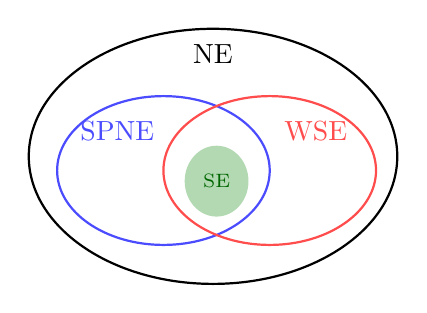
\begin{tikzpicture}[scale=0.9]
  \draw[thick] (0,0) ellipse (2.6 and 1.8);
  \node at (0,1.45) {NE};
  \draw[thick, blue!70] (-0.7,-0.2) ellipse (1.5 and 1.05);
  \node[blue!70] at (-1.35,0.35) {SPNE};
  \draw[thick, red!70] (0.8,-0.2) ellipse (1.5 and 1.05);
  \node[red!70] at (1.45,0.35) {WSE};
  \only<2->{\fill[green!50!black, opacity=0.3] (0.05,-0.35) ellipse (0.45 and 0.5);
            \node[green!40!black, font=\scriptsize] at (0.05,-0.35) {SE};}
\end{tikzpicture}
\end{column}
\begin{column}{0.48\textwidth}
\textbf{Theorem (11.3.1):} WSE $\Rightarrow$ NE
\bsk
\textbf{Theorem (11.3.2):} every finite game has a WSE
\bsk
\textbf{But:} a WSE need not be a SPNE!
\begin{itemize}
    \item Silly beliefs at unreached info sets can support silly play inside a subgame
\end{itemize}
\end{column}
\end{columns}
\vfill
{\footnotesize Bonanno Figures 11.10--11.11 give an example of a WSE that isn't a SPNE.}
\vspace{-0.2in}
\end{frame}

\begin{frame}{Coming Attraction: Sequential Equilibrium}
WSE's weak spot: \textbf{anything goes} off the path of play
\bsk
\textbf{Sequential equilibrium} (Chapter 12) adds a rule for surprises:
\begin{itemize}
    \item Pretend everyone makes tiny mistakes (``trembles'')
    \item Then every info set is reached, so Bayes' rule always works
    \item Beliefs $=$ the limit as the mistakes shrink to zero
\end{itemize}
\bsk
\textbf{Facts:} SE $\subseteq$ WSE $\cap$ SPNE. And an SE always exists
\bsk
\onslide<2->{Donut truck: SE doesn't help. Some tremble gives any $\mu$}
\vfill
{\footnotesize Not covered in this class. Kreps \& Wilson (1982, \textit{Econometrica}).}
\vspace{-0.2in}
\end{frame}

\begin{frame}{Back to Herding}
Suppose everyone guesses their own ball's color... until it stops making sense
\bsk
\textbf{Player 2} sees ``Blue'', draws blue:\\
$P(\text{Blue jar})=\dfrac{(.6)(.6)}{(.6)(.6)+(.4)(.4)}=$ \underline{\hspace{0.6in}}
\bsk
\textbf{Player 3} sees ``Blue, Blue'', draws \textbf{red}:\\
Two blue balls revealed, one red. $P(\text{Blue jar})=$ \underline{\hspace{0.6in}} \ Guess? \underline{\hspace{0.5in}}
\bsk
\onslide<2->{\textbf{Cascade:} from now on, guesses reveal nothing. Everyone herds}\\
\onslide<3->{This is Bayesian updating \textbf{along the path of play}: guesses reveal balls\\
Our groups: \underline{\hspace{0.4in}} cascades, \underline{\hspace{0.4in}} on the wrong color}
\vfill
{\footnotesize Anderson \& Holt (1997, \textit{AER}). Not in the book.}
\vspace{-0.2in}
\end{frame}

\begin{frame}{Beliefs After Surprises}
Off-path beliefs matter whenever someone does something unexpected:
\begin{itemize}
    \item \textbf{Entry:} a rival enters a market ``nobody'' would enter. Tough or desperate?
    \item \textbf{Recruiting:} a 5-star recruit decommits. Bad fit or a better offer?
    \item \textbf{Football:} going for it on 4th \& 10 at your own 20. Genius or desperate?
    \item \textbf{Earnings:} a company delays its report. Bad news?
    \item \textbf{Friends:} your always-early friend is late. Traffic or trouble?
\end{itemize}
\bsk
WSE: your answer has to be \textbf{a} belief, and your reaction has to fit it
\vspace{-0.3in}
\end{frame}

% ==============================================================
% WORKED EXAMPLE
% ==============================================================
% Answers are in the header comment.
% ---------------------------------------------------------------------

\begin{frame}[standout]
Let's Work One Out
\end{frame}

\begin{frame}{Dead Phones, Again}
Alex and Blair have dinner plans. Alex either \textbf{Cancels} (Blair knows), or goes to Cazuela's or Yoshi Sushi. Then both phones die
\bsk
\centering
\phonetree
\bsk
\raggedright
{\footnotesize Blair can't tell where Alex went: Cazuela's (C), Massey's (M), Yoshi (Y), or Home (H). Massey's is halfway, so they'd find each other. Payoffs (Alex, Blair)}
\vspace{-0.3in}
\end{frame}

\begin{frame}{Dead Phones, Again}
\begin{enumerate}
    \item Write the strategic form. Find the pure NE. Any proper subgames? \vspace{0.35in}
    \item Let $\mu=$ Pr(Cazuela's) at Blair's info set. Blair's expected payoff from C, M, Y, H? \vspace{0.35in}
    \item Which NE are part of a WSE? With what beliefs? \vspace{0.4in}
    \item If Alex mixes Cancel $\tfrac12$, Cazuela's $\tfrac13$, Yoshi $\tfrac16$: Blair's belief? Best reply? \vspace{0.2in}
\end{enumerate}
\vspace{-0.3in}
\end{frame}

\begin{frame}{What Have We Learned, Charlie Brown?}
\begin{itemize}
    \item \textbf{Assessment} $(\sigma,\mu)$: strategies plus beliefs at every info set
    \item \textbf{Sequential rationality}: best choice at every info set, given beliefs
    \item \textbf{Bayesian updating}: beliefs from $\sigma$ by Bayes' rule, when reachable
    \begin{itemize}
        \item Unreached info sets: any beliefs
    \end{itemize}
    \item \textbf{WSE} $=$ both. Kills Selten's horse's silly SPNE
    \item WSE $\Rightarrow$ NE, but not always SPNE. Fix: sequential equilibrium
\end{itemize}
\vfill
\vspace{-0.4in}
\end{frame}

\begin{frame}{Reading \& Practice}
\begin{itemize}
    \item Bonanno, Chapter 11
    \begin{itemize}
        \item \S11.1--11.3: read. Skim the $\pi_i(H\mid\sigma,\mu)$ notation
    \end{itemize}
    \item Optional: Chapter 12 for sequential equilibrium
    \item Exercises: \S11.4.1 (11.1, 11.2), \S11.4.2 (11.4), \S11.4.3 (11.6, 11.7)
    \item Solutions in \S11.5. Try them first
\end{itemize}
\vfill
\end{frame}

\end{document}
